\documentclass[a4,11pt]{pssbmac}

\usepackage[brazil]{babel}      % para texto em Português
%\usepackage[english]{babel}    % para texto em Inglês

%\usepackage[latin1]{inputenc}   % para acentuação em Português OU
\usepackage[utf8]{inputenc}   % para acentuação em Português com o uso do Unicode, 
% mude a codificação desse padrão para utf-8

%%
%% POR FAVOR, NÃO FAÇA MUDANÇAS NESSE PADRÃO QUE ACARRETEM  EM
%% ALTERAÇÃO NA FORMATAÇÃO FINAL DO TEXTO
%%
\usepackage{graphics}
\usepackage{subfigure}
\usepackage{graphicx}
\usepackage{epsfig}
\usepackage[centertags]{amsmath}
\usepackage{graphicx,indentfirst,amsmath,amsfonts,amssymb,amsthm,newlfont}
\usepackage{longtable}
\usepackage{cite}
\usepackage[usenames,dvipsnames]{color}
\usepackage{booktabs}
\begin{document}
	
	%********************************************************
	\title{Um estudo teórico-computacional de uma aplicação da Geometria de Distâncias em conformações proteicas}
	
	\author{
		{\large Guilherme Philippi}\thanks{guilherme.philippi@hotmail.com}\\
		{\small UFSC, Blumenau, SC} \\
		{\large Felipe Fidalgo}\thanks{felipe.fidalgo@ufsc.br} \\
		{\small MAT/UFSC, Blumenau, SC} \\
	}
	\criartitulo
	
	Existe uma relação muito forte com a forma geométrica das moléculas e suas funções em organismos vivos \cite{bioquimicaLehninger}, daí a importância do estudo sobre determinar estas estruturas. Nesta direção, este trabalho tem como objetivo usar a Geometria de Distâncias (GD) como modelo na conformação molecular de proteínas, em conjunto com a interpretação de dados de \textit{Ressonância Magnética Nuclear} (RMN). Como resultado, desenvolveu-se um software que facilita a construção de instâncias para testar algoritmos que se proponham a solucionar problemas fundamentais em GD \cite{carlileGDandAplications}. 
	
	A Geometria de Distâncias originou-se dos esforços de Menger (1928) \cite{menger1928}, seguido por Blumenthal (1953) \cite{blumenthal}, ao caracterizar vários conceitos da Geometria Euclidiana (como congruência e convexidade) em termos de distâncias \cite{carlileGDandAplications}. O desafio fundamental dessa área é o estudo de um problema inverso denominado Problema de Geometria de Distâncias (do inglês, DGP), onde, dados um grafo simples, ponderado positivamente e não direcionado $G=(V,E, d)$ e um inteiro $K>0$, deseja-se encontrar uma imersão $x:V\rightarrow\mathbb{R}^K$ (a qual é chamada de realização de $G$ em $\mathbb{R}^K$) tal que $\forall$ $\{u,v\} \in E$, $\left\|x(u) - x(v)\right\| = d(\{u,v\})$. 
	
	Em particular, a restrição do DGP para $k = 3$ é de interesse prático e conhecido como Problema de Geometria de Distâncias Moleculares (do inglês, MDGP), pois surgiu na busca por conformações moleculares tridimensionais --- no entanto, não é exclusivo a essa aplicação \cite{carlileGDandAplications}. Para que se crie um ambiente adequado para encontrar conformações, especificamente, para proteínas, uma relação de ordem total no conjunto $V$ foi desenvolvida \cite{carlile:MinimalOrder}. Munido de tal ordem, o espaço de busca por soluções do MDGP pode ser discretizado e, dessa forma, definindo o Problema Discretizável de Geometria de Distâncias Moleculares (do inglês, DMDGP), definido como segue \cite{carlileGDandAplications} \cite{carlileDMDGP}:
	
	\vspace{0.15cm}
	\textbf{Discretizable Molecular Distance Geometry Problem (DMDGP): } Trata-se do MDGP associado ao grafo $G = (V,E,d)$, de modo que existam um subconjunto de vértices $U_{0} = \{v_{1},v_{2},v_{3} \}$ e uma relação de ordem total $v_1, \dots, v_{|V|}$ em $V$ que satisfaça as propriedades
	\begin{enumerate}
		\item $U_{0}$ é um 3-clique em $G$;
		\vspace{-0.6cm}
		\item 
		\begin{minipage}{0.4\linewidth}  
			$\forall$ $v_{i} \in V$ tal que $i > 3$ nessa ordem:
		\end{minipage}
		\begin{minipage}{0.6\linewidth}
			\vspace{0.6cm}
			-- $U_{i} = \{v_i, v_{i-1}, v_{i-2}, v_{i-3}\}$ é um 4-clique em $G$;
			\vspace{0.2cm}
			
			-- vale a desigualdade $d_{i-3,i-1} < d_{i-3,i-2} + d_{i-2,i-1}$.
		\end{minipage}
	\end{enumerate}
	\vspace{-0.09cm}
	
	De fato, tal ordenação garante a finitude do espaço de busca por soluções \cite{carlileGDandAplications} e, além disso, organiza esse espaço, induzindo uma estrutura de \textit{árvore binária finita} --- dado que, a partir do quarto, sempre temos duas possibilidades para a realização de um vértice \cite{carlileGDandAplications}. Para tirar proveito dessa estrutura, originou-se o algoritmo chamado \textit{Branch-and-Prune} (BP) \cite{carlileDMDGP}, que consiste em uma estratégia numérica recursiva para resolver o problema eficientemente, utilizando uma busca combinatória no espaço de busca por soluções. Nele, posiciona-se vértice por vértice do grafo, seguindo a ordenação, ``podando'' todo sub-conjunto de uma solução que não respeita todas as restrições de distâncias. Especificamente, no caso proteico, essas restrições advêm tanto dos dados de RMN quanto pela geometria já conhecida das proteínas \cite{carlile:MinimalOrder}.
	
	\vspace{-0.25cm}
	\begin{figure}[h!]
		\centering
		\begin{minipage}{0.43\linewidth}   
			\paragraph{} No contexto proteico, a Ordenação de Vértices Hand-Crafted (HC) \cite{carlile:MinimalOrder} mostra-se uma boa alternativa para definir o DMDGP. Representada na Figura~\ref{fig:hcVO}, a ordenação denota um padrão repetitivo. De fato, existe uma subestrutura frequente com geometria bem conhecida nas proteínas, chamada \textit{Cadeia Principal} \cite{bioquimicaLehninger}. Mais do que discretizar o problema, a ordenação HC garante que, se as distâncias são valores precisos, o DMDGP possui apenas uma solução válida que pode ser encontrada em tempo linear.
		\end{minipage}
		\begin{minipage}{0.563\linewidth}
			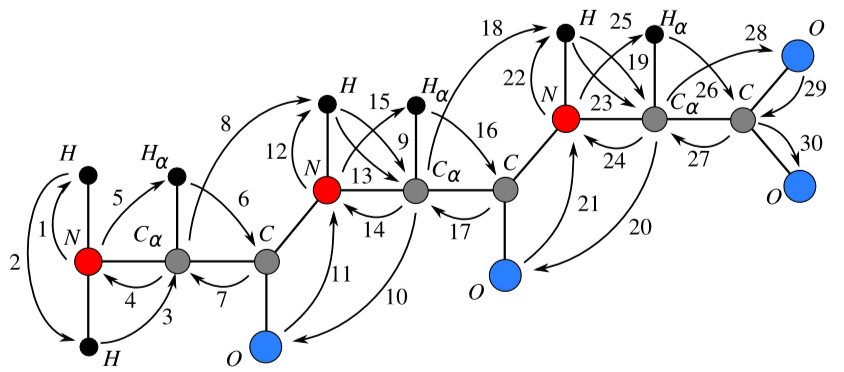
\includegraphics[scale=0.585]{hcVO.png}
			\caption{Ordenação HC \cite{carlile:MinimalOrder}.}
			\label{fig:hcVO}
		\end{minipage}
	\end{figure}
	\vspace{-0.25cm}
	
	Por fim, esse estudo teve como produto um software chamado HCProt. Seu objetivo é o processamento de dados retirados do repositório \textit{Worldwide Protein Data Bank} afim de criar instâncias esparsas (ordenadas pela HC) que podem ser usadas como entrada para implementações do algoritmo BP.  Automatiza-se, assim, a geração de instâncias DMDGP. Espera-se que este software possa auxiliar o processo de pesquisa dos autores da área. Fora implementado, também,  uma versão do algoritmo BP com o intuito de realizar simulações computacionais e, com o auxilio do software HCProt, obteve-se conformações válidas de moléculas reais. %\cite{primeiro}.
	
	\vspace{-0.14cm}
	\section*{Agradecimentos}
	O presente trabalho foi realizado com o suporte financeiro do CNPq.
	
	%\vspace{-0.14cm}
	\begin{thebibliography}{00}
		
		\bibitem{blumenthal} 
		Blumenthal, L. M. {\it Theory and applications of distance geometry}.  Oxford University Press, Oxford, 1953.
		
		%\bibitem{primeiro}
		%Fidalgo, F., Castelani, E. V. e Philippi, G.: Artigo em desenvolvimento, 2020.
		
		\bibitem{carlileDMDGP} 
		Lavor, C., Liberti, L., Maculan, N., and Mucherino, A. The discretizable molecular distance geometry problem, {\it Computational Optimization and Application}, Springer,  volume 52, number 1, pages 115-146, 2012. DOI. 10.1007/s10589-011-9402-6.
		
		\bibitem{carlile:MinimalOrder}
		Lavor, C., Liberti, L., Donald, B., Worley, B., Bardiaux, B., Malliavin, T. E. and Nilges, M. Minimal NMR distance information for rigidity of protein graphs, {\it Discrete Applied Mathematics}, Elsevier, 256:91--104, 2019. DOI:10.1016/j.dam.2018.03.071.
		
		
		\bibitem{carlileGDandAplications} 
		Liberti, L., Lavor, C., Maculan, N. and Mucherino, A. Euclidean distance geometry and applications, {\it SIAM REVIEW}, Society for Industrial and Applied Mathematics,  volume 56, number 1, pages 3-69, 2014. DOI. 10.1137/120875909.
		
		\bibitem{menger1928}
		Menger, K. Untersuchungen über allgemeine Metrik, {\it Math. Ann.},  100:75--163, 1928. DOI:doi.org/10.1007/BF01448840.
		
		\bibitem{bioquimicaLehninger} 
		Nelson, D. L. and Cox, M. M. {\it Lehninger principles of biochemistry, 6th edition}.  W.H.Freeman and Company, New York, 2012.
		
		%\bibitem{Boldrini} 
		%Boldrini, J. L., Costa, S. I. R., Ribeiro, V. R. and Wetzler, H. G. {\it Álgebra Linear e Aplicações, 3a. edição}. Harbra, São Paulo, 1984.
		%
		%\bibitem{Cuminato}
		%Cuminato, J. A. and Ruas, V. Unification of distance inequalities for linear variational problems, 
		%{\it Comp. Appl. Math.}, 2014. DOI: 10.1007/s40314-014-0163-6.
		%
		%\bibitem{daSilva} 
		%Da Silva, P. L. and Freire, I. L. On the group analysis of a modified Novikov equation, 
		%{\it Interdisciplinary Topics in Applied Mathematics, Modeling and Computational Science}, 
		%Springer Proceedings in Mathematics and Statistics,  volume 117, chapter 23, pages 161-166, 2015.
		%
		%\bibitem{Diniz1}
		%Diniz, G. L. A mudança no habitat de populações de peixes: de rio a represa -- o modelo 
		%matemático, Dissertação de Mestrado, Unicamp, 1994.
		%
		%\bibitem{Diniz2}
		%Diniz, G. L., Meyer, J. F. C. A. e Barros, L. C. Solução numérica para um problema de 
		%Cauchy Fuzzy que modela o decaimento radioativo, {\it TEMA},  23:63--72, 2001. DOI:10.1007/s40314-014-0163-6.
		%
		%\bibitem{Gomes}
		%Gomes, L. T., De Barros, L. C. and Bede, B. Fuzzy differential equation in various approaches. 
		%In {\it SpringerBriefs in Mathematics}. SBMAC- Springer, 2015. ISSN: 2191-8198.
		%
		%\bibitem{Jafelice} Jafelice, R. M., Barros, L. C. and Bassanezi, R. C. Study of the dynamics of HIV under treatment considering fuzzy delay, {\it Comp. Appl. Math.}, 33:45--61, 2014.
		
		%\bibitem{Mallet}
		%Mallet, S. M. Análise Numérica de Elementos Finitos. Tese de Doutorado, LNCC/MCTI, 1990.
		
		%\bibitem{Santos} Santos, I. L. D. e Silva, G. N. Uma classe de problemas de controle ótimo 
		%em escalas temporais, {\it Proceeding Series of the Brazilian Society of Computational and 
		%	Applied Mathematics}, volume 1, 2013. DOI: 10.5540/03.2013.001.01.0177.
		
	\end{thebibliography}
\end{document}